\documentclass[conference]{IEEEtran}

\usepackage{cite}
\usepackage[pdftex]{graphicx}
\graphicspath{{figures/}}
\usepackage[cmex10]{amsmath}
\usepackage{algorithmic}
\usepackage{algorithm}
\usepackage{array}
\usepackage{fixltx2e}
\usepackage{stfloats}
\usepackage{url}
\usepackage{amssymb}
\usepackage{float}
\usepackage{color}
\usepackage{balance}

\newcommand{\norm}[1]{\left\lVert #1 \right\rVert}

\begin{document}

\title{Parallel Stochastic Gradient Descent for Stacked Denoising Autoencoders}

\author{\IEEEauthorblockN{Jason Liang}
\IEEEauthorblockA{jasonzliang@utexas.edu}
\and
\IEEEauthorblockN{Keith Kelly}
\IEEEauthorblockA{keith@ices.utexas.edu}}

\maketitle

\begin{abstract}
We implement stacked denoising autoencoders, a special neural network that is capable of learning powerful representations of high dimensional data. Learning for autoencoders is accomplished via stochastic gradient descent and we show experimental results when training autoencoders on a standard image classification dataset. 
\end{abstract}

\begin{figure}[h]
\centering
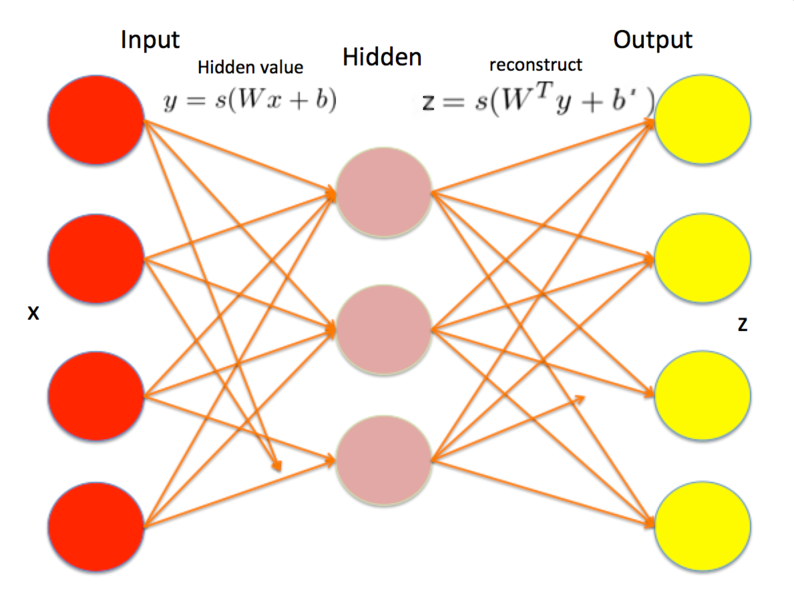
\includegraphics[width=0.9\linewidth]{autoencoder.png}
\caption{Overview of an autoencoder and its encoding, decoding stages. The weight matrix of the decoding stage is the transpose of the weight matrix of the encoding stage.}
\label{fig:autoencoder}
\end{figure}

\section{Introduction}
Autoencoders are a method for performing representation learning, an unsupervised pretraining process during which a more useful representation of the
input data is automatically determined. Representation learning is important in machine learning since ``the performance of 
machine learning methods is heavily dependent on the choice of data representation (or features) in which they are applied" 
\cite{bengio2012rep}. For many supervised classification tasks, the high dimensionality of the input data means that the classifier requires an enormous number of training examples in order to generalize well and not overfit. One solution is to use unsupervised pretraining to learn a good representation for the input data and during actual training, transform the input examples into an easier form for the classifier to learn. Autoencoders are one such representation learning tool.

An autoencoder is a neural network with a single hidden layer and where the output layer and the input layer have the same size. Consider a neural network with one hidden layer and one output layer which has the same size as the input layer. Suppose that the input $x\in\mathbb{R}^m$ (and the output as well) and suppose that the hidden layer has $n$ nodes. Then we have a weight matrix $W\in\mathbb{R}^{m\times n}$ and bias vectors $b$ and $b^{'}$ in $\mathbb{R}^m$ and $\mathbb{R}^n$, respectively. Let $s(x) = 1/(1+e^{-x})$ be the sigmoid (logistic) transfer function. Then we have a neural network as shown in Fig.~\ref{fig:autoencoder}. When using an autoencoder to encode data, we calculate the vector $y=s(Wx + b)$; corresponding when we use an autoencoder to decode and reconstruct back the original input, we calculate $z=s(W^{T}x+b^{'})$. The weight matrix of the decoding stage is the transpose of weight matrix of the encoding stage in order to reduce the number of parameters to learn. We want to optimize $W$, $b$, and $b^{'}$ so that the reconstruction is as similar to the original input as possible with respect to some loss function. In this report, the loss function used is the least squares loss: $E(t,z)=\frac{1}{2}\norm{t-z}_2^2$, where $t$ is the original input. After an autoencoder is trained, its decoding stage is discarded and the encoding stage is used to transform the training input examples as a preprocessing step. In this report, we will refer to the trained encoding stage of the autoencoder as an ``autoencoder layer".  

Usually for ordinary autoencoders, we want that $n<m$ so that the learned representation of the input exists in a lower dimensional space than the input. This is done to ensure that the autoencoder does not learn a trivial identity transformation. However, there also exists an autoencoder variant called \textit{denoising autoencoders} that use a different reconstruction criterion to learn overcomplete representations \cite{vincent2010stacked}. In other words, even if $n>m$, a denoising autoencoder can still learn a good representation of the input. This is achieved by corrupting the input image and training the autoencoder to reconstruct the original uncorrupted image. By learning how to denoise, the autoencoder is forced to understand the true structure of input data and learn a good representation of it. 

This paper, we will consider training denoising autoencoders with stochastic gradient descent (SGD). Background literature for denoising autoencoders can be found in the related work section. The algorithm description section contains more details about how SGD is implemented for autoencoders. The experiments section describes the results of training an autoencoder on a handwritten digit image dataset. Finally in future work, we discuss our plans to improve upon existing training algorithms.

\section{Related Work}
There are several papers that we'd like to mention developing the topics related to the present work. Yoshua Bengio, Aaron Courville, and Pascal Vincent review representation learning and why it is important,
single layer and deep models, autoencoders, as well as other related architectures for deep learning \cite{bengio2012rep}. For further elaboration on stacked autoencoders (and more specifically denoising autoencoders)
we refer the reader to \cite{vincent2010stacked}. Hinton et al. describe in \cite{hinton2006learning} how to successfully train deep multilayer networks, like the stacked autoencoder we use in this paper. The theory and methods behind the backpropagation algorithm that we use
is classic and can be found in \cite{hecht1989theory}. We are presently training the neural network using a stochastic gradient descent algorithm for neural networks, which is a topic covered in \cite{bottou-91c}.
Future plans include using a genetic algorithm to train the autoencoder instead of backpropagation. A survey of genetic algorithms can be found in \cite{srinivas1994genetic}.
Cant{\'u}-Paz discusses parallel genetic algorithms, which will be essentially to efficiently training our autoencoder \cite{cantu1998survey}.

\begin{figure}[h]
\centering
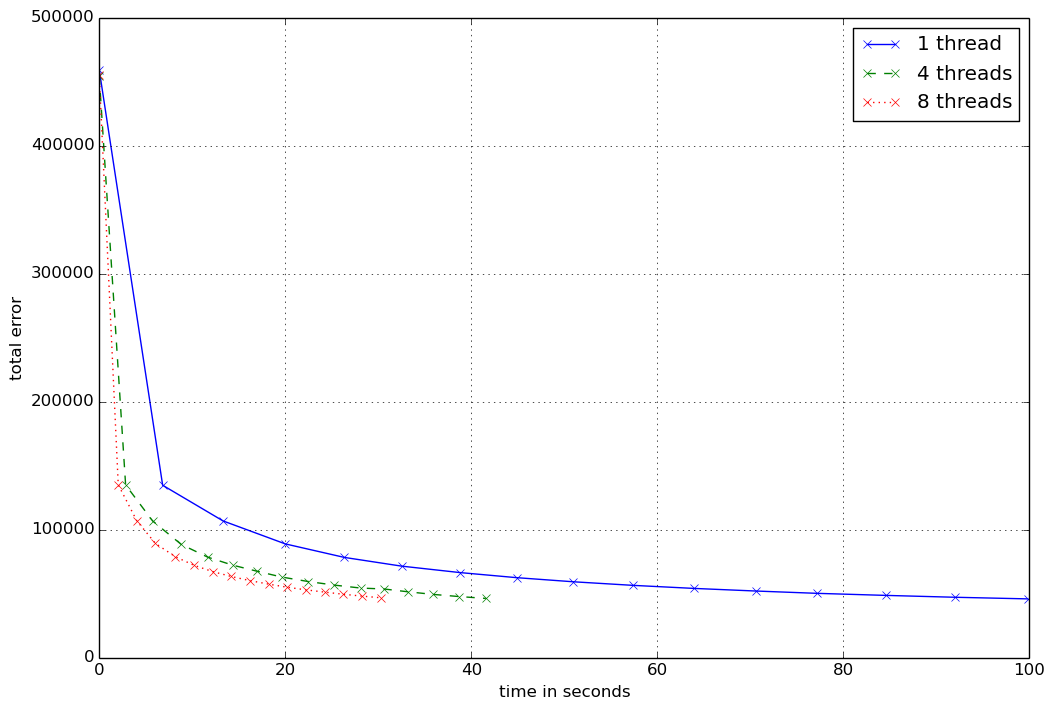
\includegraphics[width=0.9\linewidth]{experiment1.png}
\caption{Performance results on a single autoencoder layer with 500 hidden nodes and trained for 15 iterations. Plot shows time elapsed versus total training error over 5000 images for 1, 4, and 8 threads.}
\label{fig:experiment1}
\end{figure}

\section{Algorithm Description}
%todo: we need to mention that for autoencoders, the weight matrix of output layer is transpose of the weight matrix of hidden layer
%todo: also mention how autoencoders can be stacked on each other (see page 3383 in vincent2010stacked)
We start with a random weight matrix $W$ and random biases $b$ and $b^{'}$. We take a given input $x$, and feed it forward through the network and 
compute the error between the target output $t$ and the actual output $z$. Often we use the squared loss error $E(t,z) = \frac{1}{2}\norm{t-z}_2^2$ to determine the difference between the two. In the case of an autoencoder, the target output is the same as the input. If the error is not satisfactory, we can adjust the weight matrix and that biases in order to attempt to learn a better representation of the data. A common method of updating the weight and biases is via backpropogation \cite{hecht1989theory}; when applied to training inputs one at a time, it is also known as stochastic gradient descent (SGD). We will first consider the update for the weights and biases from the last hidden layer to the output layer with a squared loss error function and derive the updates. We use as an example a simple three layer neural network (one input, one hidden and one output node). Some notation:

\begin{table}[h]
\normalsize
\begin{tabular}{l|l}
Symbol     & Meaning                                                          \\ \hline
$E$          & Error as computed at the output layer                            \\
$x_j$       & Node $j$ in the input layer                                      \\
$y_j$       & Node $j$ in the hidden layer                                     \\
$z_j$       & Node $j$ in the output layer                                     \\
$n_j$       & $\sum_{i=1}^n W_{ij}x_i + b_j$                                   \\
$t_j$       & Target output at node $j$                                   \\
$W_{ij}^H$ & Weight $i,j$ from input to hidden layer \\
$W_{ij}^O$ & Weight $i,j$ from hidden to output layer \\
$s(x_j)$    & $1/(1+e^{-x_j})$                                                 
\end{tabular}
\end{table}

The derivative of the output error $E$ with respect to an output matrix weight $W_{ij}^O$ is as follows.

\begin{equation}
\begin{split}
\frac{\partial E}{\partial W^O_{ij}} &= \frac{\partial E}{\partial z_j}\frac{\partial z_j}{\partial W^O_{ij}} \\
																	 &=(z_j - t_j)\frac{\partial s(n_j)}{\partial x_j}\frac{\partial x_j}{\partial W^O_{ij}} \\
																	 &=(z_j-t_j)s(n_j)(1-s(n_j))x_i \\
																	 &=(z_j-t_j)z_j(1-z_j)x_i \\
\end{split}
\label{}
\end{equation}
Now that we have the gradient for the error associated to a single training example, we can compute the updates.
\begin{equation}
\begin{split}
\delta^O_j &= (z_j-t_j)z_j(1-z_j) \\
W^O_{ij} &\leftarrow W_{ij} - \eta \delta^O_j x_i \\
b_j &\leftarrow b_j - \eta\delta_j
\end{split}
\end{equation}

The computation of the gradient for the weight matrix between hidden layers is similarly easy to compute.
\begin{equation}
\begin{split}
\frac{\partial E}{\partial W^H_{ij}} &= \frac{\partial E}{\partial y_j}\frac{\partial y_j}{\partial W^H_{ij}} \\
																	 &=\left(\sum_{k=1}^m \frac{\partial E}{\partial z_k}\frac{\partial z_k}{\partial n_k}\frac{\partial n_k}{\partial y_j} \right)\frac{\partial y_j}{\partial n_j}\frac{\partial n_j}\partial W_{ij}^H\\
																	 &=\left(\sum_{k=1}^m (z_k - t_k)(1-z_k)z_kW_{jk}^O \right)y_j(1-y_j)x_i
\end{split}
\label{}
\end{equation}
And then using the computed gradient we can define the updates to be used for the hidden layers
\begin{equation}
\begin{split}
\delta^H_j &= \left(\sum_{k=1}^m (z_k - t_k)(1-z_k)z_kW_{jk}^O \right)y_j(1-y_j) \\
W^H_{ij} &\leftarrow W^H_{ij} - \eta\delta^H_jx_i \\
b_j &\leftarrow b_j - \eta\delta^H_j
\end{split}
\end{equation}

In general, for a neural network we may have different output error function and these will result in different update rules. We will also give the updates
for the cross-entropy error function with softmax activation in the final layer.
The cross entropy error function is given by $E(x,t) = -\sum_{i=1}^n \left(t_i\ln z_i + (1-t_i)\ln(1-z_i)\right)$
and the softmax function is given by $\sigma(x_j) = e^{x_j} /(\sum_k e^{x_k})$. Following the same procedure as above
for computing the gradient and the updates, we find that for hidden/output layer

\begin{equation}
\begin{split}
\frac{\partial E}{\partial W^O_{ij}} &= (z_j - t_j)y_i \\
\delta^O_j &= (z_j-t_j) \\
W^O_{ij} &\leftarrow W_{ij} - \eta \delta^O_j x_i \\
b_j &\leftarrow b_j - \eta\delta_j.
\end{split}
\end{equation}

Note also that we find that the updates for the hidden layer is the same as in the squared error loss function with sigmoid activation. A general overview of the backpropagation algorithm is given by by Fig.~\ref{alg:backprop}.

The algorithm and derivations for the autoencoder are a slight variation on the above derivations for a more general neural network. In particular, the weight matrix of the output layer (decoding stage) is the transpose of the weight matrix of the hidden layer (encoding stage). Thus $z=s(W^{T}(Wx + b) + b^{'})$ and $W^H_{ij} = W^O_{ji}$. We note that the steps of backpropagation can only be done in sequence; thus we can only parallelize the operations done within each step. The three major operations which benefit from parallelization are computing the matrix-vector products $Wx$ and $W^{T}y$, computing $\delta^O_j$ and $\delta^H_j$, and updating the entries of the weight matrix $W^H_{ij}$ and $W^O_{ji}$.

\begin{algorithm}[h]
\caption{Backpropogation}
\label{alg:backprop}
\begin{algorithmic}
\STATE Initialize the weights and biases randomly
\FOR{iter $=1,2,3...$}
	\FORALL{Examples $x$ in training set (randomize)}
		\STATE $z\gets$ Feedforward $x$
		\STATE Compute output layer $\delta_j^O$
		\STATE ${W_{ij} \leftarrow W_{ij} - \eta \delta^O_j x_i}$
		\STATE $b_j \leftarrow b_j - \eta\delta^O_j$
		\FORALL{Layers in reverse order}
			\STATE Compute hidden layer delta $\delta_k^H$
			\STATE ${W^H_{ij} \leftarrow W^H_{ij} - \eta\delta^H_jx_i}$
			\STATE $b_j \leftarrow b_j - \eta\delta^H_j$
		\ENDFOR
	\ENDFOR
\ENDFOR
\end{algorithmic}
\end{algorithm}

\begin{figure}[h]
\centering
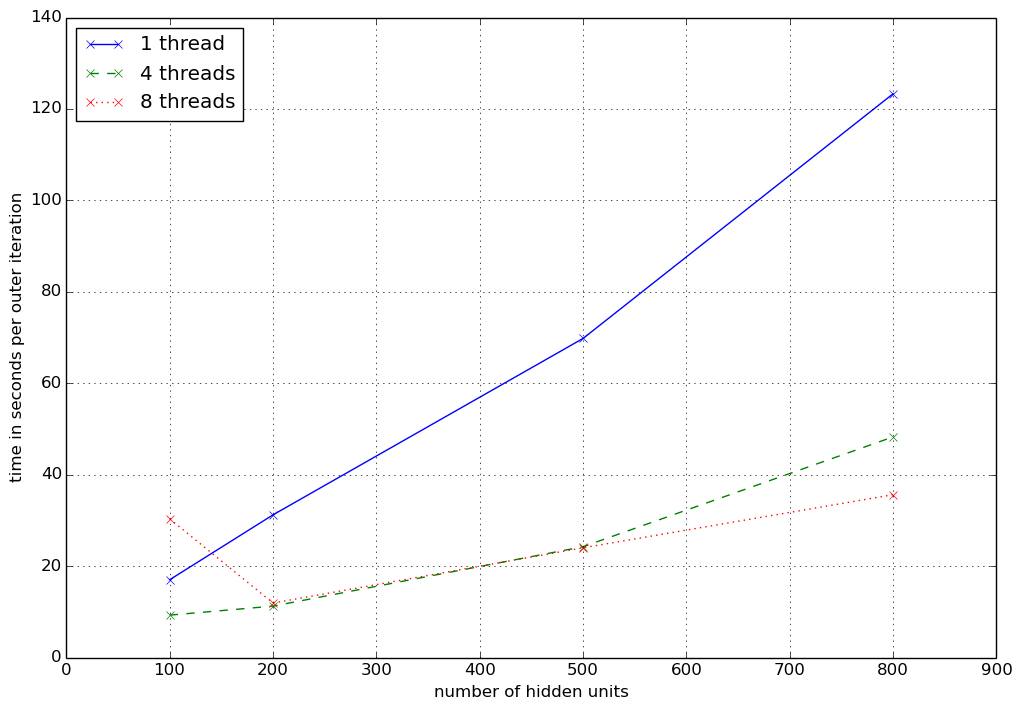
\includegraphics[width=0.9\linewidth]{experiment2.png}
\caption{Time per iteration versus number of threads and hidden nodes. All 60000 training images are used.}
\label{fig:experiment2}
\end{figure}

\section{Experimental Results}
For our experiments, we train our autoencoder over the MNIST handwritten digit dataset. The MNIST dataset is composed of 60000 training images and 10000 testing images Each image is in greyscale, is 28 by 28 pixels in size, and has a corresponding label ranging from 0 to 9. Thus, the input vector for our autoencoder has 784 dimensions. We also make use of the denoising criterion mentioned in \cite{vincent2010stacked}, and for each training image, randomly corrupt it by setting each pixel to zero with probability 0.25. 

\begin{figure}[h]
\centering
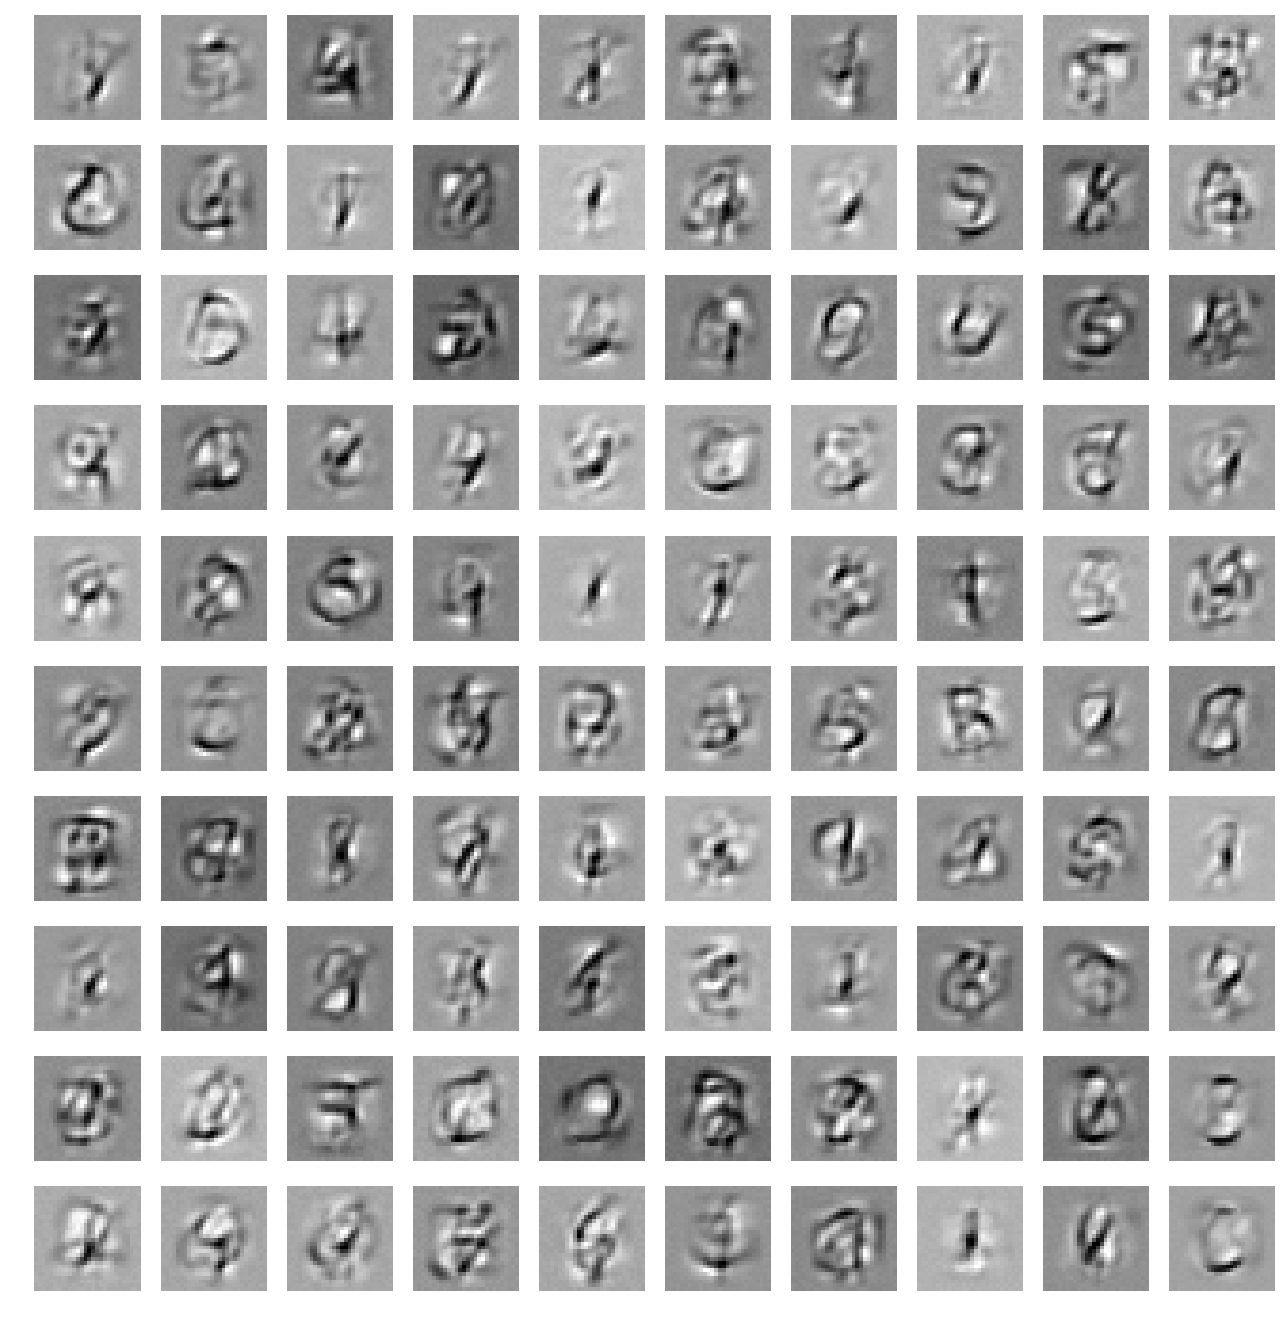
\includegraphics[width=0.8\linewidth]{experiment3_1.png}
\caption{Visualization of the filters of the first 100 hidden nodes in an autoencoder trained over all 60000 images.}
\label{fig:experiment3_1}
\end{figure}

We first analyze how the number of threads affects the rate at which training error decreases. We train a single autoencoder layer with 500 hidden nodes for 15 iterations over 5000 training images. An iteration involves going through all training images and for each image, use SGD to update the weight matrix. Fig.~\ref{fig:experiment1} shows the relationship between training error, total time elapsed, and the number of threads used. Regardless of the number of threads, the training error decreases sharply in the first few iterations before flattening out to around the same value after 15 iterations. The rate at which error decreases is significantly faster for four and eight threads when compared to just using one. Nonetheless, the speedup is not linear and is due to two reasons: 1) Possible cache conflicts as each thread read and writes to different locations in the weight matrix. 2) All the steps for backpropagation/SGD, described in Algorithm \ref{alg:backprop}, must be done sequentially. Parallelization can only be done within each step and incurs an overhead cost.

Fig.~\ref{fig:experiment2} shows the time per iteration of SGD (over all 60000 training images) versus the number of threads and hidden nodes in the autoencoder layer. For one thread, the speedup is essentially linear with the number of hidden nodes. For four threads and eight threads, the speedup becomes sublinear due to the overhead resulting from parallelization. This is especially noticeable when using eight threads and having lower number of hidden nodes; the time per iteration for eight threads with 100 hidden nodes is even slower than just using one thread. Using 8 threads only becomes faster than using four when the number of hidden nodes reach 800. 

Next, in Fig.~\ref{fig:experiment3_1}, we visualize the filters that are learned by training an autoencoder layer with 500 hidden nodes over all 60000 training images. The  filter for each hidden node is a row vector of the weight matrix and indicates which aspects of the input the hidden unit is sensitive to. Since each row in the weight matrix is the same dimensionality as the input, we can visualize it as a 28 by 28 pixel image. The filters are not identical to the input images, but do show some similarity to them. In Fig.~\ref{fig:experiment3_1}, we visualize the reconstructed digits when given noisy test digits as input. The reconstructed outputs for most of the input images are easily recognizable as digits, which indicates that the autoencoder is indeed denoising and learning a good representation of the images.

Finally we evaluate the classification accuracy of a deep neural network that has multiple stacked denoising autoencoders. We train 3 stacked autoencoder layers, each with 1000 hidden units, and using noise levels 0.1, 0.2, and 0.3 respectively. Each layer is trained for 15 iterations with a learning rate of 0.001. After the unsupervised pretraining, a conventional feedforward network with 1000 input units, 500 hidden units and 10 outputs is connected to the hidden units of the last autoencoder layer. This conventional network is then trained for 30 iterations (learning rate 0.1) in a supervised manner, where the target $t$ is the indicator vector representation of the training label. Our final classification accuracy is 98.04\%. In comparison, the accuracy achieved with a SVM with RBF kernel is 98.60\% \cite{vincent2010stacked}. 

\section{Future Work}
For future work, we plan on using a genetic algorithm (GA) to train the autoencoder's weight matrix and biases. A GA is a black-box optimization algorithm that iteratively improves upon a population of candidate solution vectors until the global optima of the objective function is reached \cite{srinivas1994genetic}. It uses operators such as mutation and crossover, which are inspired by biological evolution. GAs are superior when compared to SGD in training autoencoders in two aspects: 1) Since the loss function is highly nonconvex, SGD will always converge to a local minima, while GA are capable of eventually reaching the global optima. 2) SGD is not trivial to parallelize; as seen by our experimental results, SGD does not achieve linear speedup. On the other hand, GAs are much simplier to parallelize in one of two following ways \cite{cantu1998survey}: a) Each individual in a population can be evaluated in parallel. b) The mutation and crossover operators operate on each element of a solution vector independently and thus are embarrassing parallel.

\begin{figure}[h]
\centering
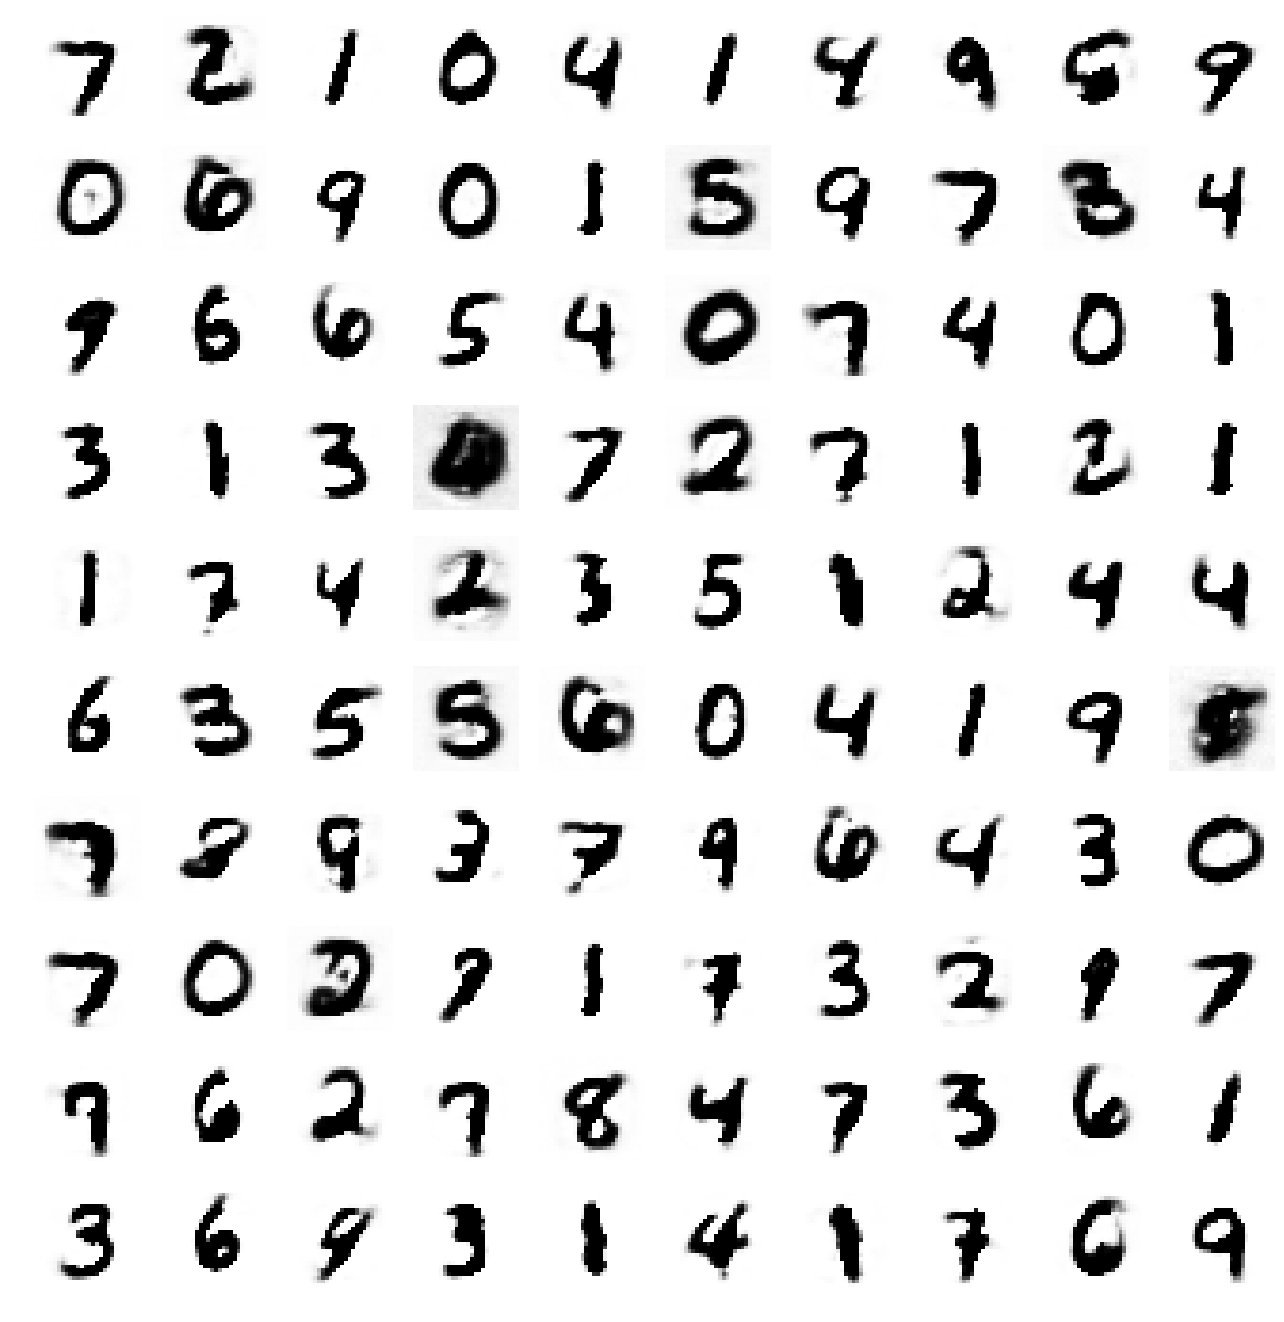
\includegraphics[width=0.8\linewidth]{experiment3_2.png}
\caption{Visualization of the reconstruction capabilities of an denoising autoencoder with 500 hidden units. Odd columns show noisy digit input images, even columns show reconstructed outputs.}
\label{fig:experiment3_2}
\end{figure}

An overview of how genetic algorithms work is given by Algorithm \ref{alg:genetic}. For autoencoders, each individual in the population is some particular weight matrix and its two associated bias vectors. The objective function would be the loss function described earlier and the fitness is how small the error outputted by the loss function is. 

We also plan on evaluating the performance of our autoencoder on additional harder image datasets mentioned in \cite{vincent2010stacked}, such as \textit{bg-rand, bg-img-rot}, which contain images with noise and rotation. 

\section{Conclusion}
We have implemented stacked denoising autoencoders and shown that it achieves accuracy comparable to state of the art classifiers like a SVM with RBF kernel. We also shown that our autoencoder layers are learning good representations and are capable of denoising and reconstructing the input with little error. For future work, we plan on exploring other optimization algorithms such as genetic algorithms for training autoencoders. 

\begin{algorithm}[h]
\caption{Genetic Algorithm}
\label{alg:genetic}
\begin{algorithmic}
\STATE Initialize $N$ individuals randomly
\FOR{iter $=1,2,3...$}
	\STATE Evaluate each individual with objective function and assign fitness.
	\STATE Create $\alpha N$ ($0 < \alpha < 1$) new individuals by selecting good individuals from population and applying mutation and crossover operators to them.
	\STATE Replace worst $\alpha N$ individuals in population with newly created individuals.
\ENDFOR
\end{algorithmic}
\end{algorithm}

\bibliographystyle{unsrt}
\bibliography{autoencoder}

\end{document}


